\documentclass[UTF8,zihao=-4,fontset=none]{ctexart}

\usepackage[a4paper,top=2.6cm,bottom=2.6cm,left=2.8cm,right=2.8cm]{geometry}
\usepackage{amsmath,amssymb}
\usepackage{booktabs}
\usepackage{array}
\usepackage{tabularx}
\usepackage{longtable}
\usepackage{graphicx}
\usepackage{subcaption}
\usepackage{float}
\usepackage{xcolor}
\usepackage{enumitem}
\usepackage{fancyhdr}
\usepackage{hyperref}
\usepackage{xurl}
\usepackage{tikz}
\usepackage{pgfplots}
\usepackage[most]{tcolorbox}

\pgfplotsset{compat=1.18}
\graphicspath{{../presentation/lung_ct_class_report/assets/}{../ppt/assets/}}

\setCJKmainfont{Songti SC}
\setCJKsansfont{Songti SC}
\setCJKmonofont{Songti SC}

\definecolor{ReportBlue}{HTML}{1E2BFA}
\definecolor{ReportInk}{HTML}{111111}
\definecolor{ReportMuted}{HTML}{5F6368}
\definecolor{ReportRule}{HTML}{D8DDF8}
\definecolor{ReportBg}{HTML}{F7F8FF}
\definecolor{ReportGreen}{HTML}{059669}
\definecolor{ReportRed}{HTML}{DC2626}

\hypersetup{
  colorlinks=true,
  linkcolor=ReportBlue,
  citecolor=ReportBlue,
  urlcolor=ReportBlue,
  pdftitle={肺部 CT 结节检测与可视化系统课程大作业报告},
  pdfauthor={组11}
}

\pagestyle{fancy}
\fancyhf{}
\lhead{\small 肺部 CT 结节检测与可视化系统}
\rhead{\small 医学图像处理课程大作业}
\cfoot{\thepage}
\setlength{\headheight}{14pt}
\setlist[itemize]{leftmargin=2em,itemsep=0.25em,topsep=0.25em}
\setlist[enumerate]{leftmargin=2.2em,itemsep=0.25em,topsep=0.25em}
\linespread{1.18}
\emergencystretch=3em

\newtcolorbox{summarybox}{
  colback=ReportBg,
  colframe=ReportRule,
  boxrule=0.7pt,
  arc=2pt,
  left=8pt,
  right=8pt,
  top=7pt,
  bottom=7pt
}

\newcommand{\code}[1]{\texttt{#1}}
\newcommand{\metric}[2]{\textbf{\textcolor{ReportBlue}{#1}}\,#2}

\title{\bfseries 肺部 CT 结节检测与可视化系统\\课程大作业报告}
\author{组11：梁宇凡（11223128）\quad 孔维萱（61523107）}
\date{2026 年 6 月 18 日}

\begin{document}
\maketitle
\thispagestyle{empty}

\begin{summarybox}
\textbf{报告摘要：}
本项目面向肺部 CT 影像中的结节候选检测任务，基于 C++17 实现了一套不依赖深度学习模型的传统图像处理 Pipeline。系统从 LUNA16 数据集的 \code{.mhd/.raw} 三维体数据出发，完成 HU 数据读取、肺窗显示、肺实质分割、二维频域带通增强、候选亮斑检测、跨切片三维聚合、多特征假阳性削减、结果可视化与官方标注验证。最终默认方案采用“规则过滤 + 轻量学习型线性评分 + 每例保留前 50\% 高分候选”的策略。在 LUNA16 subset8 的 88 例 CT、118 个官方结节上，最终方案相较调参基线将候选数从 12311 降至 6233，严格假阳性从 7903 降至 3965；严格召回从 69/118 轻微降至 68/118，达到较好的召回保持与假阳性削减平衡。
\end{summarybox}

\vspace{1em}
\noindent\textbf{关键词：} 肺结节检测；LUNA16；HU；肺实质分割；傅里叶变换；高斯差带通；GLCM；假阳性削减；医学图像可视化

\vspace{0.5em}
\noindent\textbf{代码仓库：} \url{https://github.com/YunfanGoForIt/lung-ct-nodule-detection}

\newpage
\tableofcontents
\newpage

\section{项目背景与任务定义}

肺癌早筛依赖对低剂量胸部 CT 中肺结节的及时发现。真实临床场景中，一例 CT 往往包含数百张切片，人工逐层浏览耗时较长；同时，血管截面、肺门结构、胸膜边界以及噪声点都会在二维切片上呈现近似结节的亮斑，给自动检测带来大量假阳性。本课程大作业的目标不是追求深度学习检测器的最高精度，而是用可解释、可复现的传统图像处理方法贯穿医学图像处理知识点，形成一条完整的工程链路。

本项目的输入为 LUNA16 公开数据集中的 \code{.mhd/.raw} CT 体数据及 \code{annotations.csv} 官方结节标注。输出包括肺窗图、肺实质掩膜、频域增强图、候选叠加图、最大密度投影（MIP）、候选特征表 \code{features.csv}，以及与官方标注匹配后的验证统计。整体任务可形式化为：给定三维 CT 体数据
\[
V(x,y,z)\in \mathbb{R},
\]
在肺实质区域内生成候选集合
\[
\mathcal{C}=\{c_i=(x_i,y_i,z_i,d_i,s_i)\}_{i=1}^{N},
\]
其中 \(d_i\) 为候选物理直径，\(s_i\) 为候选可信度评分。系统希望在尽量覆盖官方结节集合 \(\mathcal{A}\) 的同时，降低候选冗余数量和相对官方标注的假阳性数量。

\section{数据集与验证协议}

\subsection{LUNA16 数据说明}

LUNA16 是肺结节检测任务中常用的公开基准数据集，数据来自 LIDC-IDRI，提供 CT 体数据和结节中心坐标标注。本项目实际使用 subset8 作为主要实验数据，包含 88 例 CT，其中 60 例有官方阳性标注，共 118 个结节。每例 CT 由一个 \code{.mhd} 文本头文件和一个 \code{.raw} 裸二进制体素文件组成。头文件记录体数据尺寸、体素间距、空间原点、方向矩阵和对应 raw 文件名；raw 文件存储实际 CT 体素值。

\begin{table}[H]
\centering
\caption{实验数据与验证范围}
\begin{tabular}{ll}
\toprule
项目 & 内容 \\
\midrule
数据集 & LUNA16 subset8 \\
病例数 & 88 例 CT \\
有官方阳性标注病例 & 60 例 \\
官方结节数 & 118 个 \\
输入体数据 & \code{.mhd/.raw} \\
验证标注 & \code{annotations.csv}: \code{seriesuid}, \code{coordX/Y/Z}, \code{diameter\_mm} \\
主要评价指标 & 严格召回、10 mm 宽松召回、候选数、严格假阳性 \\
\bottomrule
\end{tabular}
\end{table}

\subsection{世界坐标匹配}

LUNA16 的标注坐标位于世界坐标系，而 Pipeline 输出的候选中心首先位于体素坐标系。根据 \code{.mhd} 中的 spacing、offset 和 transform matrix，候选体素坐标 \((x,y,z)\) 到世界坐标 \((X,Y,Z)\) 的转换为
\[
\begin{bmatrix}X\\Y\\Z\end{bmatrix}
=
\mathbf{o}
+
\mathbf{T}
\begin{bmatrix}
x\cdot s_x\\
y\cdot s_y\\
z\cdot s_z
\end{bmatrix},
\]
其中 \(\mathbf{o}\) 是空间原点，\((s_x,s_y,s_z)\) 是体素间距，\(\mathbf{T}\) 是方向矩阵。对每个官方结节 \(a_j\)，计算其与所有候选中心的欧氏距离
\[
D(a_j,c_i)=\left\|\mathbf{p}_{a_j}-\mathbf{p}_{c_i}\right\|_2.
\]
若最近候选满足
\[
D(a_j,c_i)\leq \frac{d_j}{2},
\]
则记为严格命中；若
\[
D(a_j,c_i)\leq \max\left(\frac{d_j}{2},10\text{ mm}\right),
\]
则记为宽松命中。严格假阳性定义为候选集合中没有落入任何官方结节半径内的候选数量。

\section{系统总体流程}

本系统按 Stage0--Stage5 组织，每一阶段均保留中间结果，便于调试、展示和误差复盘。流程如图 \ref{fig:workflow} 所示。

\begin{figure}[H]
\centering
\begin{subfigure}{0.45\linewidth}
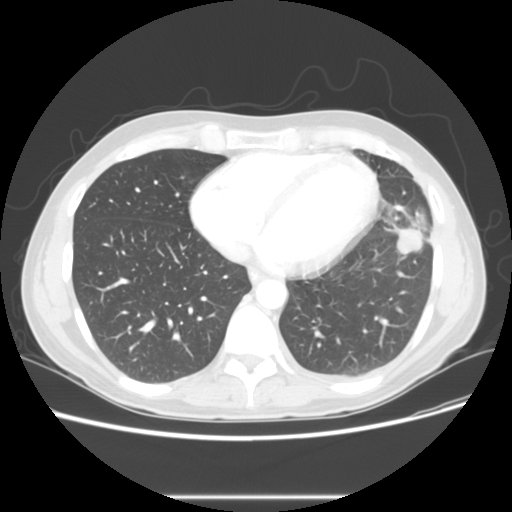
\includegraphics[width=\linewidth]{slice_window_034.png}
\caption{肺窗切片}
\end{subfigure}
\hfill
\begin{subfigure}{0.45\linewidth}

\includegraphics[width=\linewidth]{slice_mask_034.png}
\caption{肺实质掩膜}
\end{subfigure}

\vspace{0.8em}

\begin{subfigure}{0.45\linewidth}
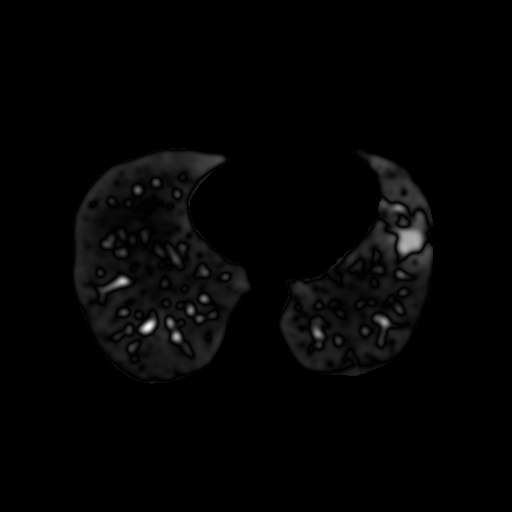
\includegraphics[width=\linewidth]{slice_bandpass_034.png}
\caption{频域带通增强}
\end{subfigure}
\hfill
\begin{subfigure}{0.45\linewidth}
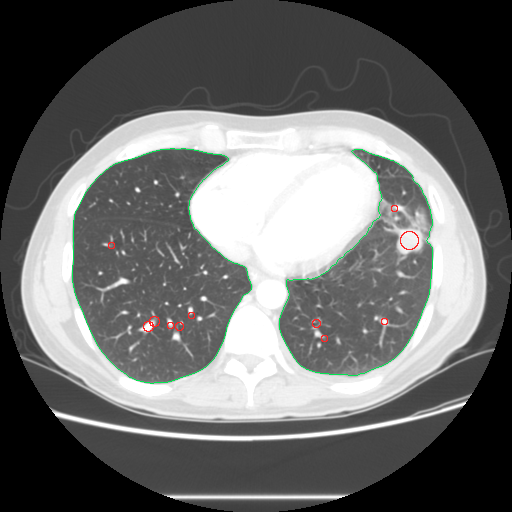
\includegraphics[width=\linewidth]{slice_overlay_034.png}
\caption{候选叠加结果}
\end{subfigure}
\caption{肺结节检测 Pipeline 的可视化中间结果：肺窗、肺实质掩膜、带通增强和候选叠加。}
\label{fig:workflow}
\end{figure}

\begin{table}[H]
\centering
\caption{Pipeline 分阶段功能}
\begin{tabularx}{\linewidth}{>{\bfseries}p{2.2cm}p{3.2cm}X}
\toprule
阶段 & 名称 & 主要功能 \\
\midrule
Stage0 & 数据读取与肺窗显示 & 解析 \code{.mhd}，读取 \code{.raw}，保留 HU 浮点体数据，输出肺窗切片和元数据。 \\
Stage1 & 肺实质分割 & 使用 HU 阈值、边界连通删除、开闭运算、最大连通域保留和空洞填充得到肺 ROI。 \\
Stage2 & 频域增强 & 对每张肺区切片做二维 FFT，使用高斯差带通突出结节尺度的中频结构。 \\
Stage3 & 候选检测 & 在肺 ROI 内根据带通响应分位阈值和 HU 范围生成种子，连通域分析得到二维候选。 \\
Stage4 & 特征筛选与评分 & 跨切片聚合为三维候选，计算形态、灰度、纹理、边界距离等特征，进行规则过滤和学习型评分。 \\
Stage5 & 验证与可视化 & 输出 \code{features.csv}、切片叠加图、MIP，并与官方标注进行距离匹配验证。 \\
\bottomrule
\end{tabularx}
\end{table}

\section{核心算法与公式}

\subsection{CT HU 读取与窗宽窗位变换}

CT 体素值采用 Hounsfield Unit（HU）表示组织对 X 射线的衰减程度。空气约为 \(-1000\) HU，水约为 0 HU，骨组织为较高正值。算法内部始终保留 HU 浮点值；显示时采用肺窗参数 \(WL=-600\)、\(WW=1500\)，将 HU 映射到 8-bit 灰度：
\[
G(x,y,z)=
\operatorname{clip}\left(
\frac{V(x,y,z)-(WL-WW/2)}{WW}\times 255,\ 0,\ 255
\right).
\]
该变换只用于显示和纹理量化，不替代原始 HU 数据。这样既保证医学强度标定不丢失，又能生成适合人工查看的肺窗图像。

\subsection{肺实质分割}

肺实质分割的目标是移除体外空气、胸壁和扫描床，将后续搜索限制在肺内。实现中首先用 HU 阈值生成低密度区域：
\[
M_0(x,y)=
\begin{cases}
1, & V(x,y,z)<-320,\\
0, & \text{otherwise}.
\end{cases}
\]
由于体外空气同样满足低 HU，随后删除与图像边界连通的低密度区域。设 \(B\) 为边界连通背景区域，则
\[
M_1=M_0\setminus B.
\]
然后进行形态学开闭运算。对结构元素 \(S\)，腐蚀与膨胀定义为
\[
M\ominus S=\{p\mid S_p\subseteq M\},\qquad
M\oplus S=\{p\mid S_p\cap M\neq \varnothing\}.
\]
开运算 \(M\circ S=(M\ominus S)\oplus S\) 用于去除小噪声；闭运算 \(M\bullet S=(M\oplus S)\ominus S\) 用于连接断裂和修正边界。最后保留面积最大的两个连通域近似左右肺，并填充肺区内部空洞，得到最终肺掩膜 \(M_{\text{lung}}\)。

\begin{figure}[H]
\centering
\begin{subfigure}{0.31\linewidth}
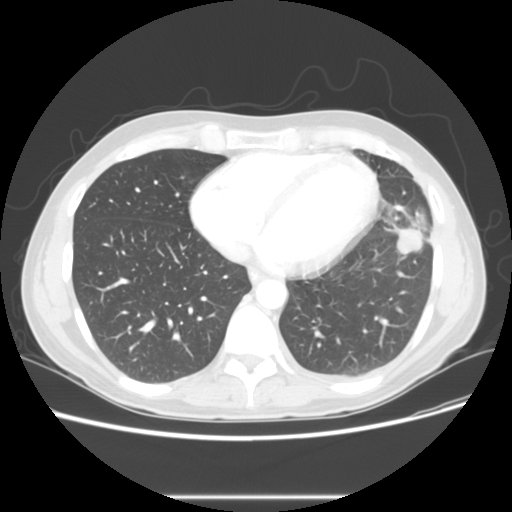
\includegraphics[width=\linewidth]{slice_window_034.png}
\caption{肺窗切片}
\end{subfigure}
\hfill
\begin{subfigure}{0.31\linewidth}

\includegraphics[width=\linewidth]{slice_mask_034.png}
\caption{肺实质掩膜}
\end{subfigure}
\hfill
\begin{subfigure}{0.31\linewidth}
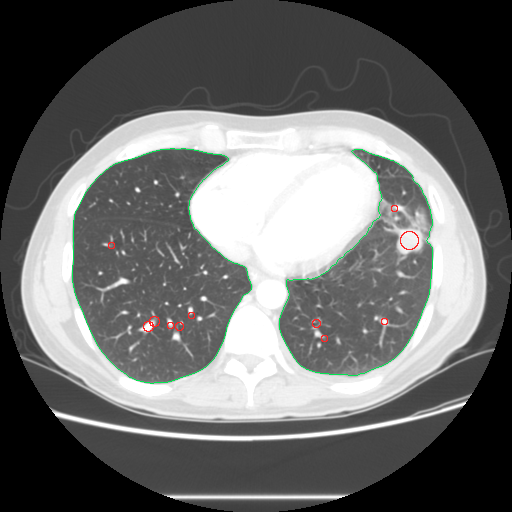
\includegraphics[width=\linewidth]{slice_overlay_034.png}
\caption{候选叠加}
\end{subfigure}
\caption{同一切片上的显示、分割与检测结果。}
\label{fig:slice-stages}
\end{figure}

\subsection{二维 FFT 与高斯差带通增强}

肺结节具有明确的物理尺度，LUNA16 中通常关注直径约 3--30 mm 的结构。大范围亮度变化和肺轮廓属于低频，噪声和细碎纹理属于高频，而结节对应相对中等尺度的局部亮结构。因此本项目对肺 ROI 内的每张切片做二维离散傅里叶变换：
\[
F(u,v)=\sum_{x=0}^{W-1}\sum_{y=0}^{H-1}
f(x,y)e^{-j2\pi(ux/W+vy/H)}.
\]
频域滤波器使用两个高斯低通响应之差构造：
\[
H(u,v)=
\exp\left(-\frac{D^2(u,v)}{2\sigma_{\text{low}}^2}\right)
-
\exp\left(-\frac{D^2(u,v)}{2\sigma_{\text{high}}^2}\right),
\]
其中 \(D(u,v)\) 为频谱点到低频中心的距离，默认 \(\sigma_{\text{low}}=30\)、\(\sigma_{\text{high}}=5\)，且 \(\sigma_{\text{low}}>\sigma_{\text{high}}\)。滤波后的图像为
\[
g(x,y)=\mathcal{F}^{-1}\{F(u,v)H(u,v)\}.
\]
该滤波器抑制大尺度背景和过细高频噪声，突出中尺度亮斑。相比理想带通，高斯差响应平滑，能减少频域硬截断带来的振铃伪影。

\begin{figure}[H]
\centering
\begin{subfigure}{0.42\linewidth}
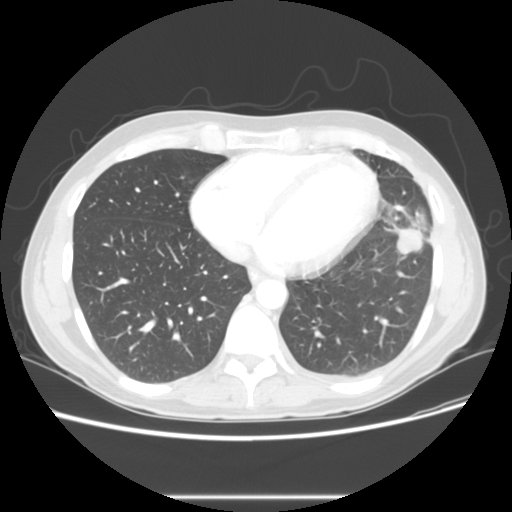
\includegraphics[width=\linewidth]{slice_window_034.png}
\caption{肺窗图像}
\end{subfigure}
\hfill
\begin{subfigure}{0.42\linewidth}
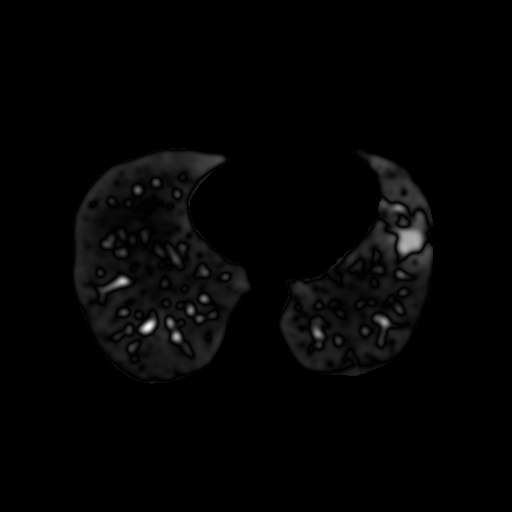
\includegraphics[width=\linewidth]{slice_bandpass_034.png}
\caption{带通增强响应}
\end{subfigure}
\caption{频域带通增强前后的视觉对比。增强图中局部中尺度亮结构更突出。}
\label{fig:bandpass}
\end{figure}

\subsection{候选亮斑检测与连通域特征}

候选生成只在肺掩膜 \(M_{\text{lung}}\) 内进行。对带通响应图 \(g\)，在肺区像素上取分位数阈值 \(T_p\)，默认 \(p=85\%\)，并结合 HU 软组织范围生成种子：
\[
S(x,y)=
\mathbb{I}\left[
M_{\text{lung}}(x,y)=1
\land g(x,y)\geq T_p
\land h_{\min}<V(x,y,z)<h_{\max}
\right],
\]
其中默认 \(h_{\min}=-500\)、\(h_{\max}=250\)。种子图经过小半径闭运算后做 8 邻域连通域分析。每个二维连通域 \(R\) 需要满足面积对应的物理直径范围，并计算下列特征：
\[
d=2\sqrt{\frac{|R|s_xs_y}{\pi}},
\qquad
\text{circularity}=\frac{4\pi |R|}{P^2},
\]
其中 \(|R|\) 是像素面积，\(P\) 是四邻域边界估计周长，\(s_x,s_y\) 为体素间距。灰度统计为
\[
\mu_{\text{HU}}=\frac{1}{|R|}\sum_{p\in R}V(p),\qquad
\sigma_{\text{HU}}=
\sqrt{
\frac{1}{|R|}\sum_{p\in R}V^2(p)-\mu_{\text{HU}}^2
}.
\]
初筛条件包括物理直径 3--30 mm、圆形度不低于 0.46、平均 HU 高于候选阶段下限等。

\subsection{GLCM 纹理特征}

为了区分实体结节和复杂血管/肺纹理，系统对候选区域的肺窗灰度图计算灰度共生矩阵（GLCM）。实现中将 8-bit 灰度量化为 16 级，并统计候选内部水平方向相邻像素对，得到归一化共生概率 \(p(i,j)\)。三个纹理特征为：
\[
\text{Contrast}=\sum_{i,j}(i-j)^2p(i,j),
\]
\[
\text{Energy}=\sum_{i,j}p(i,j)^2,
\]
\[
\text{Homogeneity}=\sum_{i,j}\frac{p(i,j)}{1+|i-j|}.
\]
其中对比度高通常意味着内部灰度变化复杂，同质性高则说明区域更均匀。最终默认规则要求 \(\text{Contrast}\leq 3.3\)、\(\text{Homogeneity}\geq 0.45\)。

\subsection{跨切片三维聚合}

二维候选只反映单层切片上的亮斑。为了得到三维候选，系统将相邻切片中中心位置接近的二维候选合并。合并后候选的 \(z\) 坐标、中心位置、直径、形态和纹理特征由组内二维候选汇总得到，并记录跨越切片数 \(\text{sliceCount}\)。该步骤能够把连续出现的结节聚合为一个三维目标，也为后续过滤单层噪声或血管截面提供特征。

\subsection{最终规则过滤与轻量学习型评分}

规则过滤用于排除明显不合理的候选，默认参数见表 \ref{tab:default-params}。它主要限制平均 HU、HU 标准差、GLCM 纹理、最大切片数和最大候选数。

\begin{table}[H]
\centering
\caption{当前默认最终方案参数}
\label{tab:default-params}
\begin{tabular}{ll}
\toprule
参数 & 默认值 \\
\midrule
\code{--min-circularity} & 0.46 \\
\code{--final-min-mean-hu} / \code{--final-max-mean-hu} & -410 / 60 \\
\code{--final-min-std-hu} / \code{--final-max-std-hu} & 25 / 210 \\
\code{--final-max-glcm-contrast} & 3.3 \\
\code{--final-min-glcm-homogeneity} & 0.45 \\
\code{--final-max-slice-count} & 18 \\
\code{--max-final-candidates} & 180 \\
\code{--learned-score-quantile} & 0.50 \\
\bottomrule
\end{tabular}
\end{table}

在规则过滤之后，候选不再只依赖硬阈值删除，而是计算一个轻量线性可信度分数。对候选 \(c\)，定义归一化特征：
\[
d_n=\frac{\operatorname{clip}(d,0,20)}{20},
\]
\[
r_n=\operatorname{clip}(\text{circularity},0,1),
\]
\[
m_n=1-\min\left(\frac{|\mu_{\text{HU}}+280|}{320},1\right),
\]
\[
s_n=\frac{\operatorname{clip}(\sigma_{\text{HU}},0,260)}{260},
\qquad
h_n=\operatorname{clip}(\text{Homogeneity},0,1).
\]
最终评分为
\[
\operatorname{score}(c)=d_n+r_n+m_n-s_n+2h_n.
\]
其设计直觉是：真实结节应大小适中、近圆、平均 HU 接近经验目标 \(-280\)、内部灰度波动较小、纹理较均匀。对每例 CT，系统按 score 从高到低排序，并保留分数排在前 50\% 的候选。这一策略比固定 top-K 更自适应：候选多的病例能显著削减冗余，候选少的病例也按自身分布保留相对可靠的目标。

\section{实验设计与调优过程}

\subsection{调参基线}

在 subset8 全量 88 例 CT 上，调参基线已经采用较合理的 HU、纹理和候选上限参数。其结果为：严格召回 69/118，10 mm 宽松召回 73/118，总候选数 12311，有标注病例严格假阳性 7903。这个基线说明系统已经能找到相当数量的官方结节，但候选数量过多，人工查看负担仍然较大。

\subsection{误差视觉分析}

对 overlay 结果进行复盘后发现，假阳性主要来自四类结构：
\begin{itemize}
  \item 血管横截面：在二维切片上近似圆形，且 HU 与真实结节接近；
  \item 血管分叉和肺门结构：局部亮斑较强，容易通过带通增强；
  \item 胸膜和肺边界附近结构：肺掩膜边界附近的小亮点会被误认为结节；
  \item 单层噪声或不稳定亮斑：在一个切片上明显，但三维连续性不足。
\end{itemize}
漏检则多发生在较淡结节、贴近肺纹理或血管的结节，以及在候选生成阶段没有形成稳定高响应亮斑的病例。该观察决定了后续调优不能只盲目收紧阈值，否则会同时删掉真实小结节。

\subsection{多方向实验}

调优过程先后测试了 3D 连续性、边界/长宽比、候选生成阈值、排序截断、固定 top-K 和学习型评分等方向。每个方向都不是孤立调参，而是对应误差分析中的一个具体假设：如果某一类假阳性确实占主导，那么加强与它相关的约束应当能在较小召回损失下减少候选。下面分别说明各方向的含义、尝试原因和结果分析，主要实验结果汇总见表 \ref{tab:all-results}。

\subsubsection{方向 A：3D 连续性过滤}

3D 连续性过滤的含义是要求最终候选至少在相邻多张切片上连续出现，例如设置 \code{--final-min-slice-count 2}，并对直径较大的候选设置例外。尝试该方向的原因是 CT 本身是三维体数据，真实结节通常具有一定体积，不应只在单张切片上出现；而很多血管横截面、孤立噪声点或边界亮点只在单层图像上形成近圆亮斑。从假阳性复盘图看，这类单层结构数量不少，因此多层连续性看起来是一个很自然的筛选条件。

实验结果表明，该方向确实显著减少了冗余候选：候选数从 12311 降到 8231，严格假阳性从 7903 降到 5460。但是严格召回从 69/118 降到 61/118，宽松召回也从 73/118 降到 65/118，损失了 8 个严格命中。原因在于 LUNA16 中存在不少小结节，受层厚、部分容积效应和带通响应强弱影响，小结节可能只在一两层上形成明显候选。硬性要求跨层连续会把单层假阳性删掉，也会把真实小结节一起删掉。因此该方向说明“三维信息有价值”，但更适合做评分特征或软约束，而不适合作为最终硬阈值。

\subsubsection{方向 B：血管与边界抑制}

血管与边界抑制主要使用两个特征：候选到肺实质边界的最小距离，以及候选二维外接框的长宽比。尝试该方向的原因来自视觉误差分析：很多误检点位于胸膜边缘、肺门附近或血管分叉区域；这些结构常常不是孤立球形结节，而更接近边界线、细长血管或复杂分叉。理论上，增加边界距离下限、限制长宽比，可以压制胸膜旁亮点和细长血管截面。

但全量结果并不理想。强过滤后严格召回降至 57/118，宽松召回降至 59/118，是所有方向中召回损失最大的；候选数只从 12311 降到 11452，严格假阳性从 7903 降到 7308，收益并不匹配损失。这说明“靠近边界”并不等于“不是结节”：临床和 LUNA16 标注中本来就有胸膜旁结节，部分结节也可能贴近血管或肺纹理。长宽比能够排除一部分细长结构，但单独用硬阈值仍然过于粗暴。后续实验中保留了“aspect ratio”作为温和辅助约束，并与候选上限组合测试，而没有继续使用较强的边界距离过滤。

\subsubsection{方向 C：候选生成阈值调整}

候选生成阈值调整发生在更早的阶段，主要改变带通响应分位数阈值和 HU 种子范围。例如提高带通响应分位数阈值，或收紧 HU 种子上限，本质上是在问：是否可以在候选池入口处减少明显不可靠的亮斑。尝试该方向的原因是，如果大量假阳性在 Stage3 就已经被带通增强选中，那么提高响应阈值应能减少后续负担；同时，过高 HU 或过低 HU 的种子也可能不是典型软组织结节。

实验结果显示，该方向收益很小。候选阈值收紧后，候选数仅从 12311 降到 12193，严格假阳性从 7903 降到 7818，但严格召回从 69/118 降到 66/118。也就是说，入口阈值稍微收紧就会丢掉一些真实结节，却几乎无法减少主要假阳性。这反映出当前假阳性并非简单的低质量噪声，而是血管、肺门和边界等“图像上确实像结节”的结构；它们同样具有高带通响应和合理 HU。另一方面，部分漏检结节在当前增强图中本来就不够突出，进一步提高阈值只会让它们更难进入候选池。因此候选生成阶段不宜继续单向收紧。

\subsubsection{方向 D：排序与固定候选截断}

排序与截断策略不改变候选生成方式，而是改变最终保留哪些候选。最初尝试限制直径奖励、惩罚单层候选，是因为旧排序分数偏好“大、圆、均匀”的候选，而血管截面也常满足这些条件。单独调整排序后，严格召回从 69/118 变为 68/118，宽松召回保持 73/118，但候选数仍为 12311，严格假阳性反而基本不变。这说明在 \code{max-final-candidates=180} 不变的条件下，只改变前 180 个候选内部排序，不能真正减少输出规模。

随后测试固定 top-K 式截断，例如 \code{max-final-candidates=120} 或 150。固定截断的含义是每例最多保留固定数量候选，它的优点是简单、可控，样本实验中也能快速减少候选数。但全量验证发现它不够稳定：cap120 将候选数降至 9115，却使严格召回降到 63/118；cap150 仍损失 4 个严格命中。原因是不同病例候选数量差异很大，固定上限会对候选多且真实结节排序靠后的病例造成更大伤害。加入 \code{aspect\_ratio <= 2.0} 后，aspect2 + cap150 成为非学习型策略中较稳的方案，严格召回 68/118、宽松召回 73/118，但候选数仍有 10576，假阳性削减幅度有限。

\subsubsection{方向 E：轻量学习型评分}

轻量学习型评分的含义是：不再用某个单一硬阈值决定候选去留，而是把直径、圆形度、平均 HU 接近度、HU 标准差和纹理同质性组合成一个线性可信度分数，再按每例候选自身分布保留前 50\% 高分候选。尝试该方向的原因是前几轮实验已经说明，硬阈值可以减少假阳性，但很容易误伤真实结节；而视觉复盘中真实结节和血管假阳性往往不是某一个特征完全不同，而是多个特征的综合差异不同。因此，用软评分表达“整体上像不像结节”比直接删除某类候选更合理。

最终学习型评分在全量 subset8 上取得最好平衡：严格召回从 69/118 小幅降至 68/118，宽松召回从 73/118 降至 71/118；候选数从 12311 降至 6233，严格假阳性从 7903 降至 3965，二者都接近减半。相较 learned top120，quantile 0.50 更适应病例差异：候选多的病例删掉低分的一半，候选少的病例也按相对可信度保留，而不是强行套用同一个固定上限。该结果说明，最终主要矛盾不是“找不到任何可疑点”，而是候选池里血管样结构过多；学习型评分能较好地把这类结构排到后半部分，同时保留大多数真实结节。

\footnotesize
\setlength{\tabcolsep}{4pt}
\begin{longtable}{p{3.25cm}>{\centering\arraybackslash}p{1.55cm}>{\centering\arraybackslash}p{1.55cm}rrp{3.1cm}}
\caption{主要优化策略对比}
\label{tab:all-results}\\
\toprule
方案 & 严格召回 & 宽松召回 & 候选数 & 严格 FP & 评价 \\
\midrule
\endfirsthead
\toprule
方案 & 严格召回 & 宽松召回 & 候选数 & 严格 FP & 评价 \\
\midrule
\endhead
baseline tuned & 69/118 & 73/118 & 12311 & 7903 & 调参基线 \\
3D 连续性硬过滤 & 61/118 & 65/118 & 8231 & 5460 & 假阳性下降但召回损失过大 \\
边界/长宽比强过滤 & 57/118 & 59/118 & 11452 & 7308 & 胸膜旁真实结节被误伤 \\
候选阈值收紧 & 66/118 & 71/118 & 12193 & 7818 & 收益很小且召回下降 \\
排名 cap/penalty & 68/118 & 73/118 & 12311 & 7904 & 单改排序不能减少数量 \\
cap120 & 63/118 & 68/118 & 9115 & 6025 & 固定截断不够稳 \\
aspect2 + cap150 & 68/118 & 73/118 & 10576 & 6814 & 非学习型最佳但降幅有限 \\
learned top120 & 68/118 & 71/118 & 9115 & 6019 & 低于 quantile 策略 \\
learned quantile 0.50 & 68/118 & 71/118 & 6233 & 3965 & 综合最佳 \\
\bottomrule
\end{longtable}
\normalsize
\setlength{\tabcolsep}{6pt}

可以看到，硬阈值过滤通常能减少候选数量，但会明显牺牲召回。固定 top-K 的问题是病例间候选数量差异较大，统一上限无法兼顾候选丰富病例和候选稀疏病例。最终选择的 learned quantile 0.50 策略则在轻微召回损失下接近砍半候选数量和假阳性。

\section{实验结果与可视化}

\subsection{最终指标}

最终方案与调参基线的核心指标见表 \ref{tab:final-results}。候选数减少
\[
1-\frac{6233}{12311}=49.37\%,
\]
严格假阳性减少
\[
1-\frac{3965}{7903}=49.83\%.
\]
严格召回仅减少 1 个结节，宽松召回减少 2 个结节。

\begin{table}[H]
\centering
\caption{调参基线与最终方案对比}
\label{tab:final-results}
\begin{tabular}{lrrrr}
\toprule
方案 & 严格召回 & 宽松召回 & 候选数 & 严格假阳性 \\
\midrule
调参基线 & 69/118 & 73/118 & 12311 & 7903 \\
最终方案 & 68/118 & 71/118 & 6233 & 3965 \\
\midrule
变化 & -1 & -2 & -6078 & -3938 \\
变化率 & -0.85 pct & -1.69 pct & -49.4\% & -49.8\% \\
\bottomrule
\end{tabular}
\end{table}

\begin{figure}[H]
\centering
\begin{tikzpicture}
\begin{axis}[
  ybar,
  width=0.94\linewidth,
  height=7.2cm,
  ymin=0,
  ymax=110,
  ylabel={百分比（\%）},
  symbolic x coords={严格召回,候选数,严格假阳性},
  xtick=data,
  bar width=12pt,
  enlarge x limits=0.22,
  legend style={at={(0.5,-0.18)},anchor=north,legend columns=3,draw=none},
  nodes near coords,
  nodes near coords align={vertical},
  every node near coord/.append style={font=\scriptsize},
  tick label style={font=\small},
  label style={font=\small},
  ymajorgrids=true,
  grid style={draw=ReportRule}
]
\addplot+[fill=ReportBlue!80,draw=ReportBlue] coordinates {
  (严格召回,58.5) (候选数,100.0) (严格假阳性,100.0)
};
\addplot+[fill=ReportGreen!70,draw=ReportGreen] coordinates {
  (严格召回,57.6) (候选数,85.9) (严格假阳性,86.2)
};
\addplot+[fill=ReportRed!70,draw=ReportRed] coordinates {
  (严格召回,57.6) (候选数,50.6) (严格假阳性,50.2)
};
\legend{调参基线,非学习型最佳,最终学习型方案}
\end{axis}
\end{tikzpicture}
\caption{召回保持与冗余削减的综合对比。严格召回使用对 118 个官方结节的命中率；候选数与严格假阳性使用相对调参基线的比例。}
\label{fig:metric-bars}
\end{figure}

\begin{figure}[H]
\centering
\begin{tikzpicture}
\begin{axis}[
  width=0.92\linewidth,
  height=7cm,
  xlabel={每例保留策略},
  ylabel={数量},
  symbolic x coords={baseline,cap150+aspect2,learned top120,learned q0.50},
  xtick=data,
  x tick label style={rotate=15,anchor=east},
  ymin=0,
  legend style={at={(0.5,-0.22)},anchor=north,legend columns=2,draw=none},
  ymajorgrids=true,
  grid style={draw=ReportRule},
  mark options={solid}
]
\addplot+[ReportBlue,very thick,mark=*] coordinates {
  (baseline,12311) (cap150+aspect2,10576) (learned top120,9115) (learned q0.50,6233)
};
\addplot+[ReportRed,very thick,mark=square*] coordinates {
  (baseline,7903) (cap150+aspect2,6814) (learned top120,6019) (learned q0.50,3965)
};
\legend{候选数,严格假阳性}
\end{axis}
\end{tikzpicture}
\caption{不同后处理策略下候选数与严格假阳性的下降趋势。}
\label{fig:candidate-trend}
\end{figure}

\subsection{可视化输出}

系统输出的可视化图像包括肺窗切片、肺掩膜、带通响应、红色候选叠加图和 MIP。图 \ref{fig:mip} 展示了最大密度投影结果，能从整体上观察候选空间分布；切片叠加图则适合逐例定位误差来源。

\begin{figure}[H]
\centering
\begin{subfigure}{0.45\linewidth}
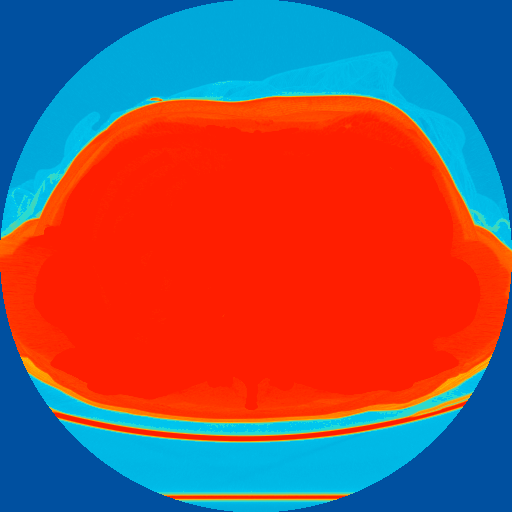
\includegraphics[width=\linewidth]{mip.png}
\caption{基线 MIP}
\end{subfigure}
\hfill
\begin{subfigure}{0.45\linewidth}
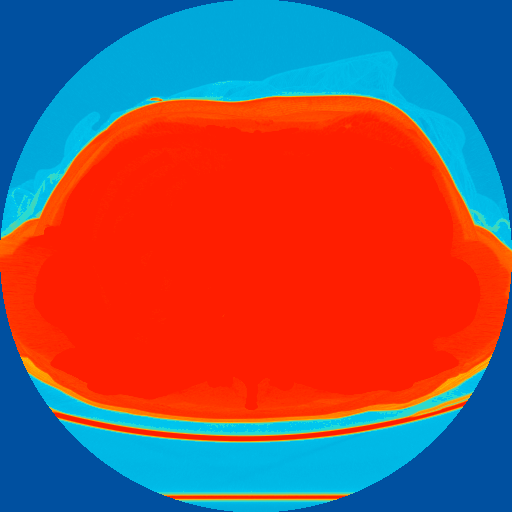
\includegraphics[width=\linewidth]{mip_tuned.png}
\caption{调优后 MIP}
\end{subfigure}
\caption{MIP 可视化结果对比。伪彩色投影有助于观察候选在三维空间中的分布。}
\label{fig:mip}
\end{figure}

\section{工程实现与复现方式}

工程采用 C++17 实现核心 Pipeline，Make/CMake 负责构建。命令行程序 \code{build/lung\_pipeline} 接收一个 \code{.mhd} 文件和输出目录，默认启用最终推荐参数。核心输出包括：
\begin{itemize}
  \item \code{meta.txt}：体数据尺寸、spacing、窗宽窗位、带通参数、候选阈值和评分策略；
  \item \code{features.csv}：候选 ID、中心体素坐标、直径、圆形度、HU 统计、GLCM 特征、边界距离、长宽比和切片数；
  \item \code{slice\_XXX\_window.pgm}：肺窗切片；
  \item \code{slice\_XXX\_mask.pgm}：肺实质掩膜；
  \item \code{slice\_XXX\_bandpass.pgm}：频域带通增强图；
  \item \code{slice\_XXX\_overlay.ppm}：肺轮廓与候选叠加图；
  \item \code{mip.ppm}：伪彩色最大密度投影。
\end{itemize}

构建与基本测试命令如下：
\begin{verbatim}
make
make test
\end{verbatim}
真实数据运行命令如下：
\begin{verbatim}
./build/lung_pipeline path/to/case.mhd output/case_result
\end{verbatim}
与 LUNA16 官方标注验证：
\begin{verbatim}
./tools/validate_luna_annotations.py \
  --mhd path/to/case.mhd \
  --features output/case_result/features.csv \
  --annotations data/luna16_zenodo/csv/annotations.csv \
  --out output/case_result/annotation_validation.csv
\end{verbatim}
全量 subset8 批处理：
\begin{verbatim}
./tools/run_subset_batch_validation.py \
  --subset-dir data/luna16_subset8_download/subset8 \
  --annotations data/luna16_zenodo/csv/annotations.csv \
  --output-root data/subset8_batch_validation_final_default \
  --pipeline ./build/lung_pipeline
\end{verbatim}

\section{讨论与局限}

本项目的优点是链路完整、可解释性强、调参过程可复现。每个候选都可以追溯到肺窗图、掩膜、带通响应、连通域特征和最终评分，适合作为医学图像处理课程大作业展示。最终学习型评分虽然带有“学习”思想，但本质仍是基于人工候选特征的线性评分，不依赖深度学习或预训练模型，因此能够清楚体现灰度变换、形态学、频域滤波、连通域分析和纹理特征等课程知识点。

主要局限如下：
\begin{itemize}
  \item 血管截面与实体小结节在二维图像上高度相似，传统形态和纹理特征仍难以完全区分；
  \item 部分漏检发生在候选生成阶段，后处理评分无法恢复没有进入候选池的真实结节；
  \item 学习型评分主要基于 subset8 的候选特征搜索，虽然做了 train/test split 观察，但样本量有限，仍可能存在过拟合；
  \item LUNA16 官方标注是结节中心点和直径，并非逐像素分割 mask，因此严格假阳性统计应理解为相对官方标注的候选冗余；
  \item 当前 Pipeline 以传统图像处理为主，若追求临床级性能，还需要引入更强的三维上下文建模、候选分类器或深度学习检测网络。
\end{itemize}

\section{结论}

本课程大作业完成了一套基于传统图像处理的肺部 CT 结节检测与可视化系统。系统能够从 LUNA16 原始 \code{.mhd/.raw} 体数据出发，端到端完成 HU 读取、肺实质分割、频域带通增强、候选检测、三维聚合、多特征筛选、官方标注验证和可视化输出。通过多轮误差分析和调优，最终采用轻量学习型评分策略，在 subset8 全量 88 例 CT 上将候选数和严格假阳性接近减半，同时仅损失 1 个严格命中。该结果说明，在不使用深度学习的前提下，合理结合医学图像先验、频域增强、形态纹理特征和数据驱动的轻量评分，仍然可以构建一个完整、可解释、可复现的肺结节候选检测系统。

\appendix
\section{源码与材料索引}

\begin{table}[H]
\centering
\caption{报告使用的主要项目材料}
\small
\begin{tabularx}{\linewidth}{>{\raggedright\arraybackslash}p{5.4cm}X}
\toprule
文件 & 用途 \\
\midrule
\texttt{README.md} & 项目简介、默认参数、运行方式和最终指标。 \\
优化探索报告.md & 多轮调参过程、误差分析、各策略全量指标。 \\
肺部CT结节检测大作业设计文档-2.md & 原始设计思路、算法分阶段说明。 \\
\path{include/lung_pipeline.h} & Pipeline 参数结构、候选特征结构和默认配置。 \\
\path{src/lung_pipeline.cpp} & 肺分割、FFT 带通、候选检测、GLCM、学习型评分等核心实现。 \\
\path{tools/validate_luna_annotations.py} & 体素坐标到世界坐标转换和官方标注匹配逻辑。 \\
\path{presentation/lung_ct_class_report/assets/} & 报告复用的可视化图像素材。 \\
\bottomrule
\end{tabularx}
\normalsize
\end{table}

\section{最终方案命令行参数}

\begin{verbatim}
--min-circularity 0.46
--final-min-mean-hu -410
--final-max-mean-hu 60
--final-min-std-hu 25
--final-max-std-hu 210
--final-max-glcm-contrast 3.3
--final-min-glcm-homogeneity 0.45
--final-max-slice-count 18
--max-final-candidates 180
--learned-score-quantile 0.50
\end{verbatim}

\end{document}
